\documentclass[tikz,border=2pt]{standalone}
\usepackage{amsmath}
\usepackage{amssymb}
\definecolor{bgcol}{HTML}{171D2B}
\definecolor{accent}{HTML}{F7B538}
\definecolor{linecol}{HTML}{CBD5E1}
\definecolor{muted}{HTML}{94A3B8}
\pagecolor{bgcol}
\color{white}
\begin{document}
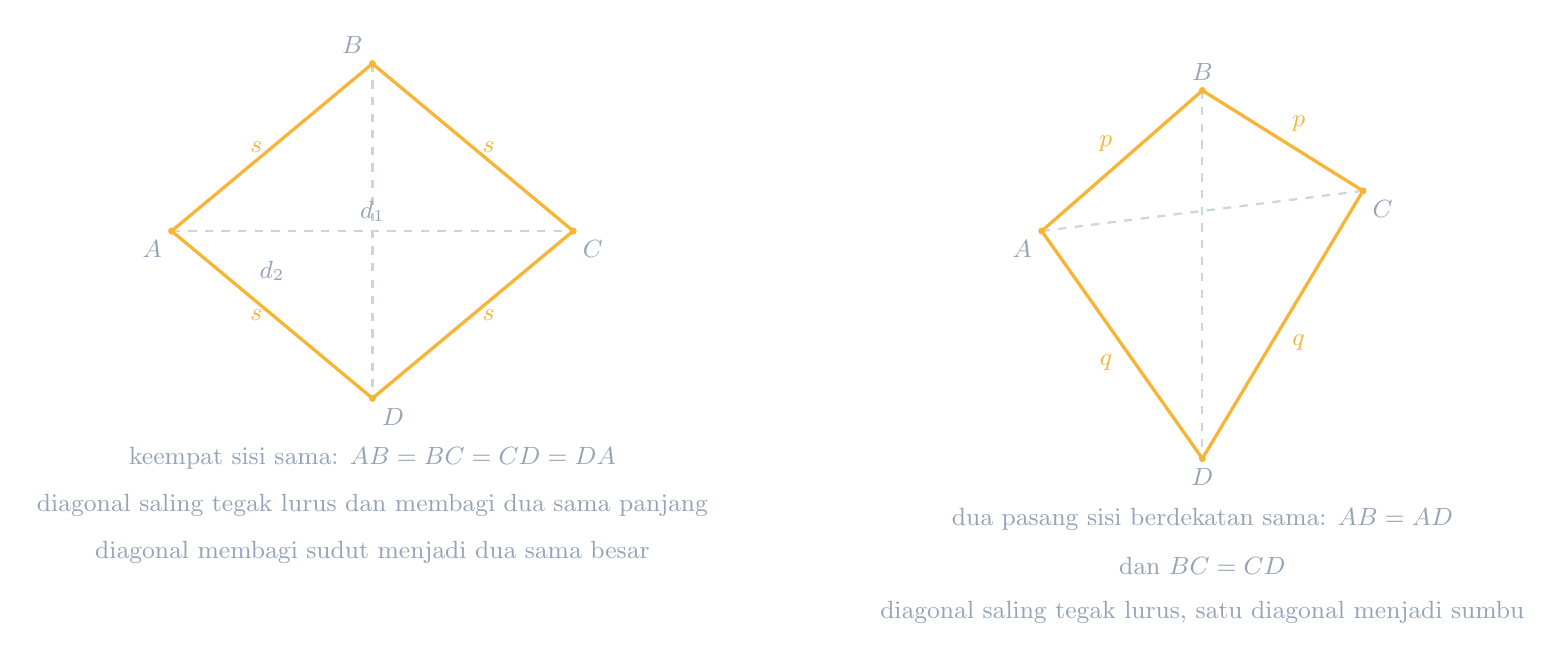
\begin{tikzpicture}[scale=0.85,>=stealth]
  % ===== Belah ketupat =====
  \coordinate (A) at (0,0);
  \coordinate (B) at (3,2.5);
  \coordinate (C) at (6,0);
  \coordinate (D) at (3,-2.5);
  \draw[very thick,accent] (A) -- (B) -- (C) -- (D) -- cycle;
  \draw[thick,linecol,dashed] (B) -- (D);
  \draw[thick,linecol,dashed] (A) -- (C);
  \fill[accent] (A) circle (1.5pt) (B) circle (1.5pt) (C) circle (1.5pt) (D) circle (1.5pt);
  \node[below left,muted] at (A) {\small $A$};
  \node[above left,muted] at (B) {\small $B$};
  \node[below right,muted] at (C) {\small $C$};
  \node[below right,muted] at (D) {\small $D$};
  \node[left,accent] at (1.5,1.25) {\small $s$};
  \node[right,accent] at (4.5,1.25) {\small $s$};
  \node[right,accent] at (4.5,-1.25) {\small $s$};
  \node[left,accent] at (1.5,-1.25) {\small $s$};
  % diagonal labels
  \node[above,muted] at (3,0) {\small $d_1$};
  \node[below,muted] at (1.5,-0.3) {\small $d_2$};
    \node[muted] at (3,-3.4) {\small keempat sisi sama: $AB=BC=CD=DA$};
  \node[muted] at (3,-4.1) {\small diagonal saling tegak lurus dan membagi dua sama panjang};
  \node[muted] at (3,-4.8) {\small diagonal membagi sudut menjadi dua sama besar};
  % ===== Layang-layang =====
  \begin{scope}[xshift=13cm]
    \coordinate (A) at (0,0);
    \coordinate (B) at (2.4,2.1);
    \coordinate (C) at (4.8,0.6);
    \coordinate (D) at (2.4,-3.4);
    \draw[very thick,accent] (A) -- (B) -- (C) -- (D) -- cycle;
    \draw[thick,linecol,dashed] (A) -- (C);
    \draw[thick,linecol,dashed] (B) -- (D);
    \fill[accent] (A) circle (1.5pt) (B) circle (1.5pt) (C) circle (1.5pt) (D) circle (1.5pt);
    \node[below left,muted] at (A) {\small $A$};
    \node[above,muted] at (B) {\small $B$};
    \node[below right,muted] at (C) {\small $C$};
    \node[below,muted] at (D) {\small $D$};
    \node[above left,accent] at (1.2,1.05) {\small $p$};
    \node[above right,accent] at (3.6,1.35) {\small $p$};
    \node[below left,accent] at (1.2,-1.7) {\small $q$};
    \node[below right,accent] at (3.6,-1.4) {\small $q$};
    \node[muted] at (2.4,-4.3) {\small dua pasang sisi berdekatan sama: $AB=AD$};
    \node[muted] at (2.4,-5.0) {\small dan $BC=CD$};
    \node[muted] at (2.4,-5.7) {\small diagonal saling tegak lurus, satu diagonal menjadi sumbu};
  \end{scope}
\end{tikzpicture}
\end{document}
